\documentclass[../main.tex]{subfiles}
\graphicspath{{\subfix{../images/}}}
\begin{document}
	
	\chapter{The test- and characterization procedure}
		\section{Developing the characterization procedure}
		One goal of this work is to develop an experimental procedure, to characterize the camera that may be flown on the STEP mission. This characterization is crucial to test the validity of the scientific goals for the mission and should cover the metrics outlined in the preceding chapter. Such a procedure should be exactly reproducible, such that we can ensure its correctness. In this chapter, the initial considerations and the results from preliminary tests will be described. The conclusion that leads to the final measurement plan will then be presented.
		
		\subsection{The initial experimental setup for test plan development}
		The camera described in table \ref{table:testcam} was used in the development of this testing and characterization procedure. The initial setup to carry out the testing and characterization procedure is seen in figure \ref{fig:setup}. 
		
		\begin{figure}
			\centering
			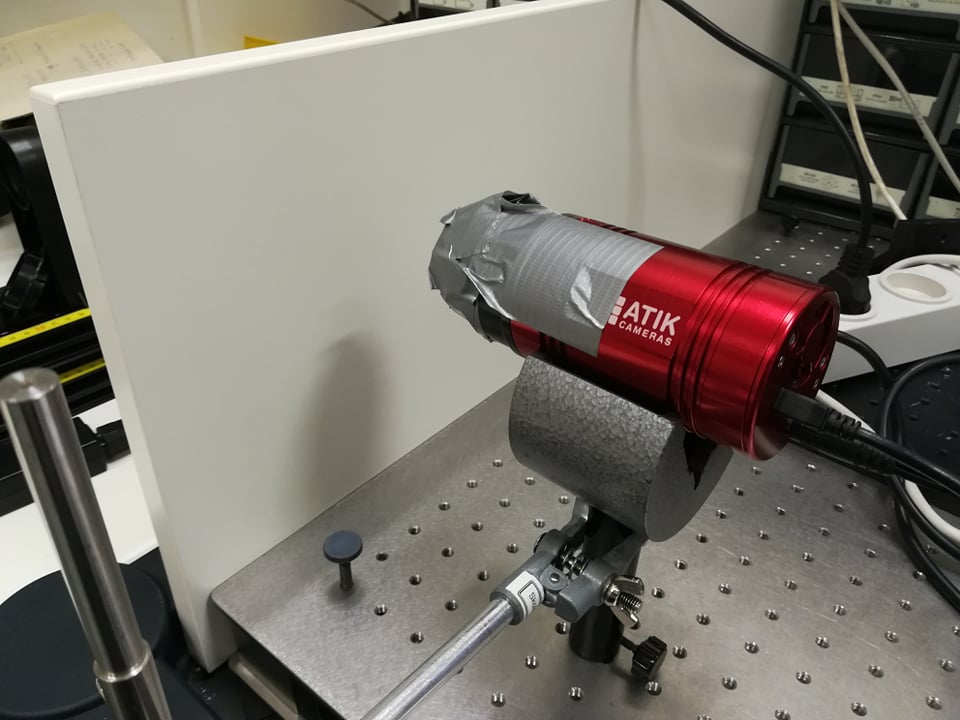
\includegraphics[width=0.6\textwidth]{setup.jpg}
			\caption{The initial experimental setup used both for the light and dark exposures. The setup consists of the test procedure camera resting on a stand. The camera is pointed into a white lacquered wooden screen, connected via USB2 to a lab computer, and a power supply. The setup is placed in a dark room to ensure we can acquire a proper dark frame.}
			\label{fig:setup}
		\end{figure}
		
		The setup consists of the camera resting on a stand, pointed into a white lacquered wooden screen. The camera is connected via USB2 to the lab computer and a power supply. Since the setup for dark frames requires a sufficiently dark room, an in-house darkroom is used.
		For all light exposures, the ambient room lighting was used, with the camera pointed into the screen. The ambient light is a double fluorescent bulb, and the light can be dimmed to roughly half of the flux by turning off half the bulbs. This is useful in order to control the length of exposure times during the acquisition of linearity data. To focus the light, and avoid rapid over-saturation, a pinhole was constructed from heavy black cardboard and mounted with tape.
		For all dark frames, the same configuration was used, but with no ambient light, and computer screens turned off. 
		
		\begin{table}[]
			\centering
			\begin{tabular}{|c|c|}
				\hline
				\textbf{Model name }& Atik 414EX mono \\
				\textbf{Chip name}& Sony ICX 825\\
				\textbf{Readout noise (typical)}& 5$e^-$\\
				\textbf{Gain factor}& 0.28$e^-$/ADU\\
				\textbf{Cooling $\Delta T$}& $-30^\circ$\\
				\textbf{Dark current}& $\sim 0.001 e^-\;$ at $\;-10^\circ$ \\
				\textbf{ADC}& 16 bit\\
				\textbf{Pixel size}& $6.45 \mu m \times 6.45 \mu m$\\ 
				\textbf{Shutter}&No\\
				\hline
			\end{tabular}
		\caption{Relevant data specs for the \textbf{Atik 414EX mono} camera \cite{atik414specs}}\label{table:testcam}
		\end{table}
			
		\subsection{Preliminary thoughts and considerations}
		The starting point for the development of an experimental procedure will be outlined in this section. This is then tested experimentally, and from these results, the final procedure will be described. 
		
		\subsubsection{Acquiring data and reducing noise}
		Characterization of a CCD chip involves acquiring images in a variety of ways to study several effects. Here, practical noise reduction steps that should be applied, will be described. 
		
		We acquire frames while varying a parameter like temperature (for thermal noise) or exposure time (for linearity). For each value of this varied parameter, say temperature for thermal noise (dark current), we wish to associate a functional value. In the case at hand, it is electrons per second. This is done by considering the frame taken at that value of the variable (temperature), and computing the mean value of the experimental metric (dark current, electrons per second) across all pixels in the image. For any measurement, we should take steps to reduce the noise in the image. Dark current can be reduced by cooling the chip before acquiring data frames. Readout noise is \textbf{gaussian} and the noise in the distribution is reduced by a factor of $1/\sqrt{N}$ for $N$ measurements. Hence, for each datapoint, before computing the desired variable, like dark current for a specific temperature, we should, at that temperature, acquire $N$ frames, and construct a mean image from these $N$ frames. Typically $N$ is chosen to be as large as is practically feasible. The value of the experimental metric is then computed from that average frame. Initially, $N = 100$ was chosen, but since, at ambient lighting levels used for the linearity measurements, longer exposure times make this impractical, $N=10$ was chosen instead. The difference in the functional behavior of the curve, as a result of choosing a smaller value of N, was found to be of little importance. The temperature was chosen to be $T = -10^\circ$ C, due to reasons outlined in the next section.
	
		\subsubsection{Background noise and dark current}
		A good starting point for the development of the testing procedure originates from a preliminary investigation of the noise levels of the chip. This test was carried out at a desktop in an office, using a very primitive experimental setup. This preliminary test confirms that dark current is strongly dependent on temperature. See figure \ref{fig:dcprelim}. Since the camera cooler can cool to a temperature gradient of $\Delta T = 30 ^\circ $C, the temperature $T = -10 ^\circ$ C was chosen. Since the cooling system works as a temperature gradient, it is not feasible to go much lower. These steps ensure that we can minimize dark current and read-out noise.
		\begin{figure}
			\centering
			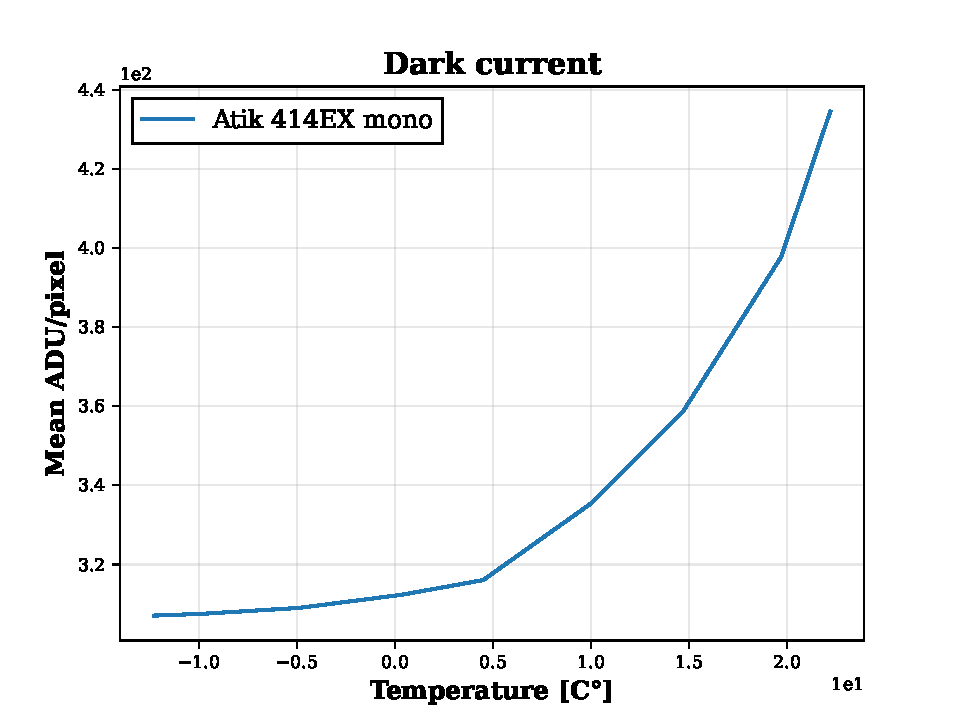
\includegraphics[width=0.6\textwidth]{dark_current_versus_temperature.pdf}
			\caption{Preliminary dark current measurement, performed at the office in sub-optimal settings, to get a first glimpse of the behavior of this variable.}
			\label{fig:dcprelim}
		\end{figure}
		
		\subsubsection{Master bias and flat field frames}
		Bias images are frames with the smallest possible exposure time. This exposure time is $0.001s$ for the test procedure camera. Thus, for the construction of the master bias frame, we may choose $N$ as large as$N = 300$.  The bias frames are acquired in a dark setting with no light. This frame should be subtracted from all other data points. The same repeat number is chosen for the master flat-field frame, where the exposure time was chosen to be $10s$.  The flat-field frames are acquired in a lit room setting. 
		
		For both the bias frames and the flat-field frames, we choose the $T= -10^\circ$ temperature setpoint chosen above, to reduce dark current.
		
		\subsubsection{Exposure times for linearity}\label{sec:explin}
		The linearity measurement consists of acquiring exposures of the white screen, as a function of exposure time, in order to study the linearity of the response in measured photons by the detector. Hence we should first determine which exposure time interval to use. At first, a 100s exposure acquisition was carried out, in which considerable saturation was observed. From this, it was concluded that an exposure time of 100 seconds was a good datapoint to use for the last acquisition. This is true for the configuration in which all light bulbs were turned on in the room, representing the maximal flux achievable with this setup. The choice of exposure times generally relies on trial and error, to decide what range of exposure times we should use, at a given light source intensity. At first frames at exposures between $0.001s$ and $10s$ in $1s$, between $10s$ and $100$s in $10s$ intervals, and $100s$ and $110s$ in $1s$ intervals was acquired. It was found that the light source stability varies slightly, resulting in greater uncertainty in short exposure measurements, and hence it was chosen to omit $0.001$ seconds, and instead acquire frames in the interval $1s$ to $10s$ in 1-second intervals, in addition to the data sequence described just above. Due to the impracticality due to time constraints, of performing many measurements at long exposure times, it was instead chosen to acquire frames in the interval $10s$ to $110s$ in $5s$ intervals, which also samples the non-linearity curve better. Measurements with exposure times shorter than $10s$ are found to be more uncertain, see figure \ref{fig:linearity}, likely due to a time offset resulting from the lack of shutter on the testing camera. The time calibration in question, which will be described below, poses difficulties. Hence it is recommended that a dimmer light source is used, and instead, frames are acquired at longer exposure times that pose lesser uncertainty in the measurements. 
		
		\begin{figure}
			\centering			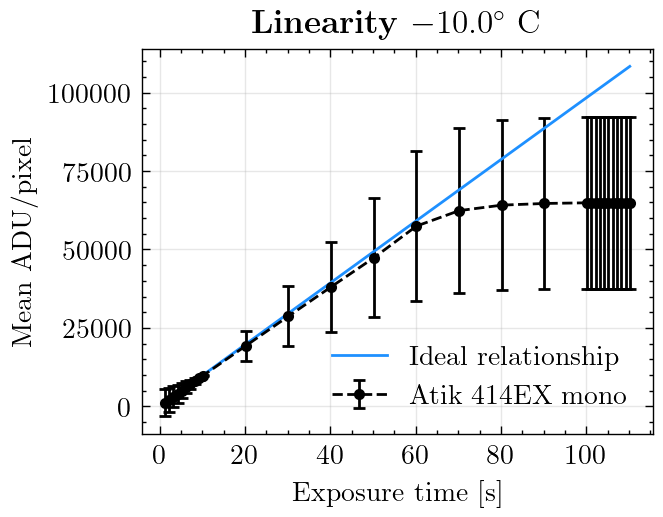
\includegraphics[width=0.65\textwidth]{linearity.png}
			\caption{A plot of the percentage deviation from ideal linearity, computed according to equation  \ref{eq:fluxcorrect_timecal} for each exposure time after meaning across $N$ frames. }
			\label{fig:linearity}
		\end{figure}
		
		\subsubsection{Noise as a function of temperature}
		Readout noise and dark current are expected to be temperature-dependent, and hence, in the entire cooling range of the camera,  images of dark frames were acquired in order to study the behavior of these physical effects. Exposure times are chosen such that the minimal exposure time is chosen for the readout noise images since no photon should have been detected, and since the dark current is time-dependent, and hence should be negligible in this regime. For dark current frames, it is crucial to pick an exposure time such that the dark current contribution is greater (by a considerable amount, higher orders of magnitude) than the readout noise contribution. Dark current follows a \textbf{poissonian} distribution, and to recover this underlying distribution we should pick long exposure times. Since this requires \textbf{very} long times of exposure, it is more practical to pick an exposure time of $10s$, and then mean over $N = 100$ acquired images at this temperature, to reduce the noise contribution, since readout noise should be Gaussian with a zero-centered mean value. 
		
		\begin{figure}
			\centering			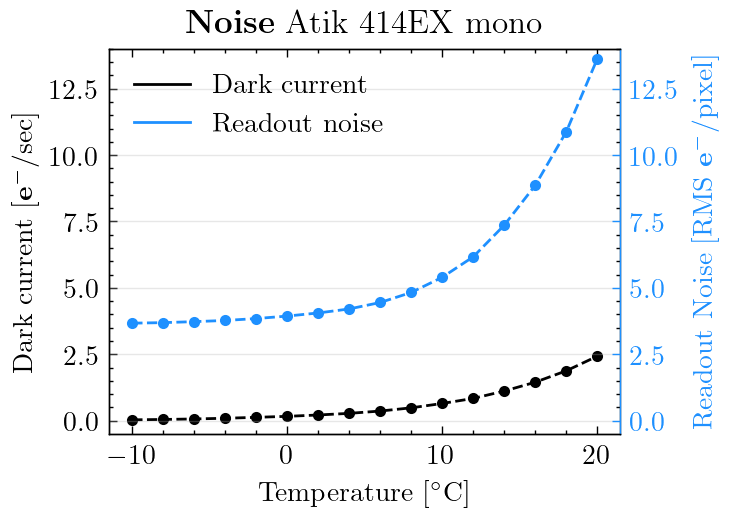
\includegraphics[width=0.65\textwidth]{noise_versus_temperature.png}
			\caption{Dark current and readout noise as a function of temperature. The datapoints have been constructed by acquiring 100 dark frames at exposure times $0.001$ s for readout noise, and $10$s for dark current, at each temperature. Readout noise is computed according to section \ref{sec:rondc}, and dark current according to equation \ref{darkcurrenteq}. }
			\label{fig:noise}
		\end{figure}
		
		\subsubsection{Hot pixel treatment}
		It is crucial to treat hot pixels. One way to do this is to realize that hot pixels are those pixels in which dark current does not show a linear temporal behavior. Acquiring a \textit{very} long exposure, here chosen as a $1000s$ exposure, and a medium-long (considerably shorter than the former) exposure, here chosen to be a $90s$ exposure, we can study the dark current in each pixel, and determine if there is a linear relationship between the two frames. 
		
		Small values of the dark current are most accurately measured in the long exposure image, while the short exposure image will allow for the large dark current values to be accurately measured. We can not that for the test procedure camera, readout noise at $T = -10^\circ$C, is around 3-4 electrons per image. Dividing that by the exposure time in the short exposure image, $90s$, corresponds to a dark current of about $0.33-0.44 e^-/\text{sec}$. It was noted that the dark current contribution should be significantly greater, for us to be able to see the Poissonian distribution of the thermal noise. Thus we may conclude that the smallest measurable dark current in that image will be around twice that \cite{bibid}. We use this value as a filter, below which we do not include the pixel in the following treatment. 
		
		By scatter plotting the pixels in the short exposure against the same pixels in the long exposure, and finding (qualitatively) the range within which the data points seem to follow a nice linear relationship. The remainder, that is those above a certain threshold beyond which they no longer appear to be linear, are considered hot in this sense, and from this information, a mask can be constructed. For the test procedure camera, this value is around a dark current of $7.5 e^-/$sec. These pixels are then marked, and an image mask is formed. This mask marks which pixels to omit in the other analysis.
		
		\subsubsection{Testing of ground assumptions}
		In our experimental setup, assumptions have been made that need to be tested. The two most important ones, which enable the testing of linearity are that 
		\begin{itemize}
			\item The camera has a well-calibrated zero-point temporally. That is to say that a 10-second exposure is physically the frame resulting from light being able to enter the chip for exactly 10 seconds. This is of particular importance since the camera used for the development of the testing procedure does not have a shutter.
			\item The ambient light source in the room is stable during exposure, so we can accurately compare ADU intensities between different frames. The ambient room light is used, which consists of double fluorescent light bulbs. We should as a null hypothesis expect to find fluctuations, and potentially even drifts in the light source over time.
		\end{itemize}
		The latter assumption can be tested by analyzing the many exposures taken during the first linearity sequence, by plotting the percentage deviation, from the mean ADU (mean across all $N=100$ exposures at a given exposure time) as a function of exposure time. Both of these tests are outlined in the following two sections. 
		
		\subsection{Stability of the lightsource}
		The experimental setup assumes the ideal case of a stable light source. This assumption should be tested, since we can generally not expect a fluorescent light bulb, connected to the main relay, to be stable to high precision. Preliminary investigations may utilize the wealth of data acquired during the linearity measurement sequence. At each exposure interval, $N = 100$ repeat frames were recorded. This enables us to plot the intensity as a function of time. From each repeat series, a mean image can be constructed. The mean ADU/pixel in this image is our reference value. The percentage deviation in the mean ADU/pixel, in each of the individual repeat frames, was then plotted as a function of time. This makes it possible to qualitatively judge the stability of the light source as a function of time. Such a plot can be seen in figure \ref{fig:lightsourcestability}. Save for a few of the exposure times, the lighting is only stable to a few percentage points deviation. This yields a first estimate of the instability, indicating that we should correct this source of systematic error. 
		
		\begin{figure}
			\centering			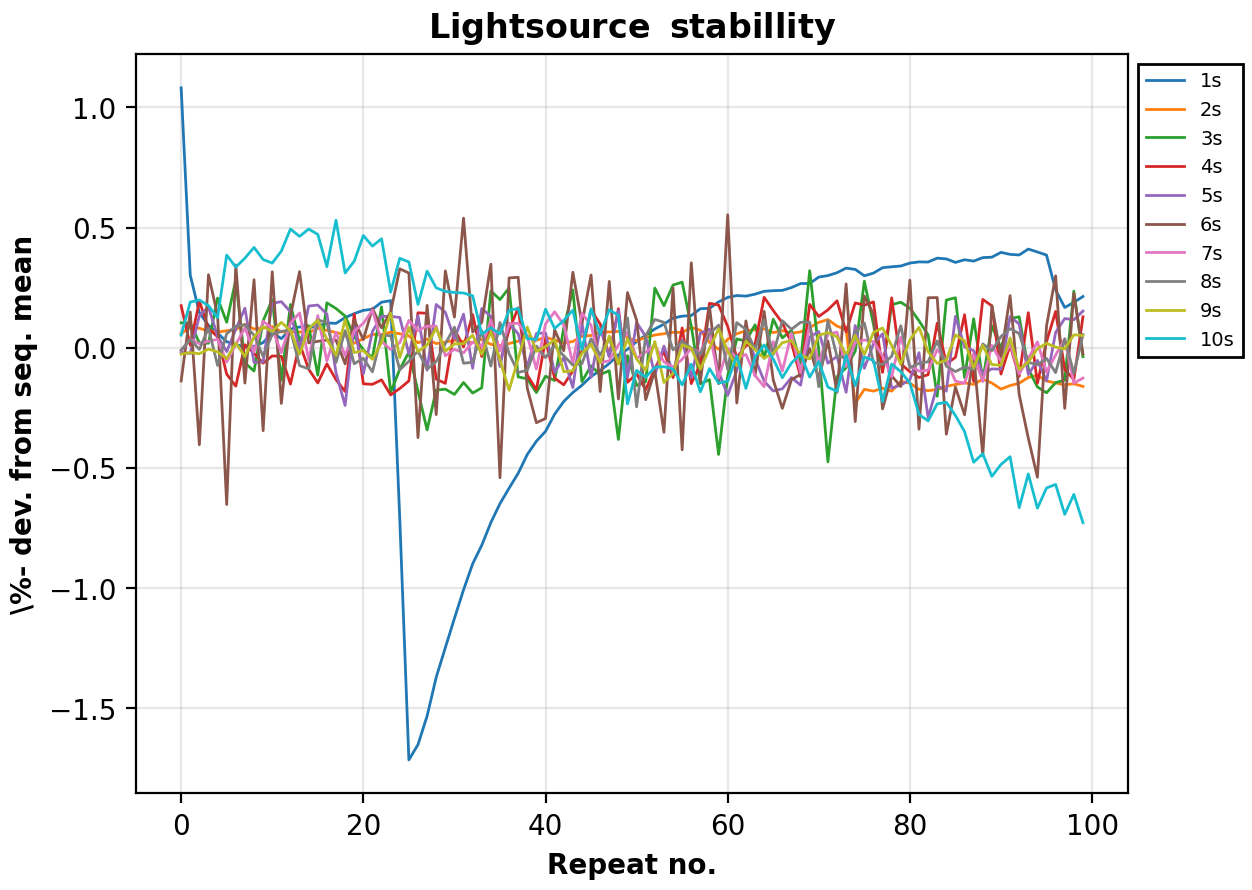
\includegraphics[width=0.8\textwidth]{lightsource.png}
			\caption{A plot of the temporal dependence in the lightsource intensity (flux) across each of the different exposure times. Numbering is ordered according to the preliminary series of exposure times as described in the text.}
			\label{fig:lightsourcestability}
		\end{figure}
		
		These deviations from perfect stability cannot be used as a correction, since this does not include the correlation of instability between exposure times. Instead, it is proposed that a reference exposure be utilized. Within a given repeat sequence, one may use a reference of $10s$ exposure by alternating between the chosen reference exposure, and the desired exposure time. Such an exposure series is akin to $[10s, 1s, 10s, 1s, 10s, \dots 10s, 2s, 10s, 2s,\dots]$ covering the entire range of exposure times. For each frame, we then have a 10-second exposure just before and right after. For the test procedure camera, the software designed for the camera only enables the user to set up a sequence of 10 data points to be acquired automatically but allows that sequence to be repeated. Hence it was most practical for the analysis to acquire data in the series $[10s, 1s, 10s, 2s, 10s, 3s, 10s, \dots 10s, 9s, 10s]$, repeat that N times, and then repeat until the desired exposure time range has been covered. $N=10$ was chosen due to time constraints. The two reference measurements to use in the correction of a given frame will then be the two taken at adjacent times. 
		
		The flux of the light source at the time of our desired frame then lies somewhere in between, assuming no wild fluctuations or drifts, and a linear change in the time in between acquisition of the two reference frames. These assumptions of local monotonicity of the light source flux are justified by considering figure \ref{fig:lightsourcestability}. In this way we are also able to correct for the potential long temporal drift of the intensity. Let $\bm F(x[s]) = \text{mean}\left(\text{Image}([s])\right)$ be interpreted as the mean flux in an image of exposure time $s$ in seconds, that is, the mean ADU value of an arbitrary image of exposure time $s$. Hence we may correct for the instability, using a 10 second reference exposure, for a given frame via the computation
		\begin{equation}\label{eq:fluxcorrect_notimecal}
			\bm F(x [s])_\text{corrected} = \frac{\bm F(x [s])}{\frac12\left[\bm F(10s)_\text{before}+\bm F(10s)_\text{after}\right]} * 10,
		\end{equation}
		where the last factor of 10 is to account for the relation between the 10 seconds and 1 second exposure times, in the ideal case where there is no time offset.
		
		\subsection{Time calibration}
	Another assumption to be tested pertains to the camera itself: the time calibration of the measurements. A series of measurements were constructed to study if the zero-point was actually at $0s$ and to what precision. A preliminary estimate is gained by acquiring eight frames, noting that, under the assumption that our detector is linear, it should be true that for a given frame $\text{Image}(\text{Exposure time})$, we must expect for a perfect time calibration that 
	
	\begin{equation}
		\frac{\text{Image}(21s) - \text{Image}(1s)}{\text{Image}(11s) - \text{Image}(1s)} = \frac{\text{Image}(10s) - \text{Bias}}{\text{Image}(20s) - \text{Bias}}
	\end{equation}
	Or that 
	\begin{equation}
		\frac{\textbf{mean}(\text{Image}(21s) - \text{Image}(1s))}{\textbf{mean}(\text{Image}(11s) - \text{Image}(1s))} - \frac{\textbf{mean}(\text{Image}(10s) - \text{Bias})}{\textbf{mean}(\text{Image}(20s) - \text{Bias})} = 0,
	\end{equation}
	where \textbf{mean}$()$ refers to the mean ADU/pixel within an image. The result of this, for the test procedure camera, being $0.0063$ indicates a time offset which must be determined properly, and applied as a correction. The test procedure camera does not have a shutter, and the data sheet \cite{atik414specs}, specifies a $1/15 s$ readout time. Hence an exposure time of $1s$ should correctly be interpreted as an exposure time of $1s + \Delta t$, where $\Delta t$ should be deduced experimentally. Via a seperate linearity measurement series with greater precision (more datapoints) in the uncertain interval of $1s - 10s$, see figure \ref{fig:timecal} in which this readout time would actually be able to significantly impact exposure times, we can get a first estimate of $\Delta t$ by fitting a linear function to the data points, and determining the roots of polynomium. 
	\begin{figure}
		\centering			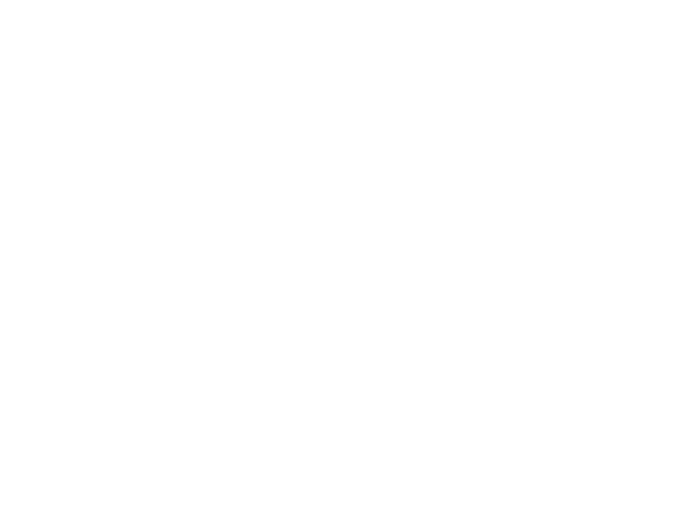
\includegraphics[width=0.65\textwidth]{time_calibration.png}
		\caption{}
		\label{fig:timecal}
	\end{figure}
	If there is a time offset, the line will intersect the first axis at a point different from the origin. The intersection point on the first axis should be subtracted. For a negative value of the intersecting point on the first axis, a subtraction physically corresponds to a longer exposure time. In the same figure, the corrected data points are shown, along with the fit to the corrected data (in red). Deviations from the initial linear fit may be seen in figure \ref{fig:timecaldev}, once again indicating that shorter exposure times are more uncertain. 
	
	\begin{figure}
		\centering			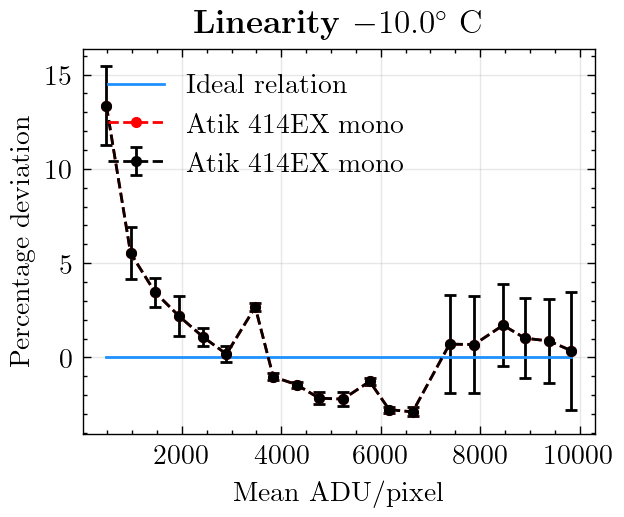
\includegraphics[width=0.65\textwidth]{time_calibration_deviations.png}
		\caption{}
		\label{fig:timecaldev}
	\end{figure}
	Since we still observe fluctuations in the low exposure regime, we may try to circumvent the issue of fluctuations by using $1s$ exposure frames as a reference, by instead acquiring one $2s$ frame, "sandwiched" (in time) by two reference measurements of $1s$ exposure. Let us define $\bm F_A, \bm F_B$ to be the flux of the $1s$ reference frames that are taken respectively before and after the $2s$ frame, and correspondingly $\bm F_2$ the flux of the $2s$ frame. In that case the relation between the mean value of the flux before and after, to that of the flux of the $2s$ frame, which should be divided by $2$ to correct for the double exposure time, multiplied by the \textit{true} exposure times, should be equal to unity
	\begin{align}
		\frac{\frac12(\bm F_A + \bm F_B) (1+\Delta t)}{
			\frac12 \bm F_2 (2+\Delta t)} &= 1\\
		\intertext{Or, rearranging a bit, canceling the factors of $1/2$ and isolating for $\Delta t$ yields}
		% \frac{(\bm F_A + \bm F_B)}{\bm F_2} + \Delta t \frac{(\bm F_A + \bm F_B)}{\bm F_2} &= 2+\Delta t\\
		% \frac{(F_A + F_B)}{F_2} - 2 &= \Delta t \left(1- \frac{(F_A + F_B)}{F_2}\right)\\	
		\Delta t = 	\frac{(\bm F_A + \bm F_B) / \bm F_2 - 2}{1- (\bm F_A + \bm F_B)/ \bm F_2} \label{eq:timecalprec}
	\end{align}
	
	We should then correct for this time offset by adjusting the equation \ref{eq:fluxcorrect_notimecal}, and achieving the same time the true measure of non-linearity, $\delta$ by subtracting $1$ and converting to percentages as 
		\begin{equation}\label{eq:fluxcorrect_timecal}
		\delta = \left( \frac{\bm F(x [s])}{\frac12\left[\bm F(10s)_\text{before}+\bm F(10s)_\text{after}\right]}\frac{10s + \Delta t}{x [s] + \Delta t} - 1 \right) * 100\%.
		\end{equation}
		
		\subsection{Linearity}
		The non-linearity, defined by equation \ref{eq:fluxcorrect_timecal}, for data acquired in exposure times according to section \ref{sec:explin}, may be seen in figure \ref{fig:linearity}. Consider the same figure, but zoomed in in figure \ref{fig:linearityzoom}. Perfect linear behavior is plotted as a blue line. Glancing at the graph we see there is an ADU interval, from around $0$ to $45000$ ADU, with the exception of a couple of datapoints, namely the first and the sixth. Whether the sixth datapoint is a statistical outlier, or a true peculiarity of the non-linearity curve, should be determined by a repeat of the experiment. Once again, fluctuations are observed in the low ADU regime, here corresponding to short exposure times in the interval between 1 seconds to 10 seconds. The latter is used as the reference exposure, which is why it correctly displays zero deviation. We may investigate if this is due to an incorrect estimate of the time offset, by varying it. 
		In order to get a more precise estimate of the time offset from equation \ref{eq:timecalprec}, we may, after correcting, interpret \ref{eq:fluxcorrect_timecal} as the true non-linearity, recognizing the low ADU datapoint deviations as imprecise. Fitting a linear curve to the data in figure \ref{fig:linearityzoom}, gives us a best estimate of the \textit{true} linearity at the faulty points, which can be used to correct the fluxes in equation \ref{eq:timecalprec}. This yields a new time offset, that may be reinserted in our analysis, and this process may be iterated until convergence. 
		
		\begin{figure}
			\centering			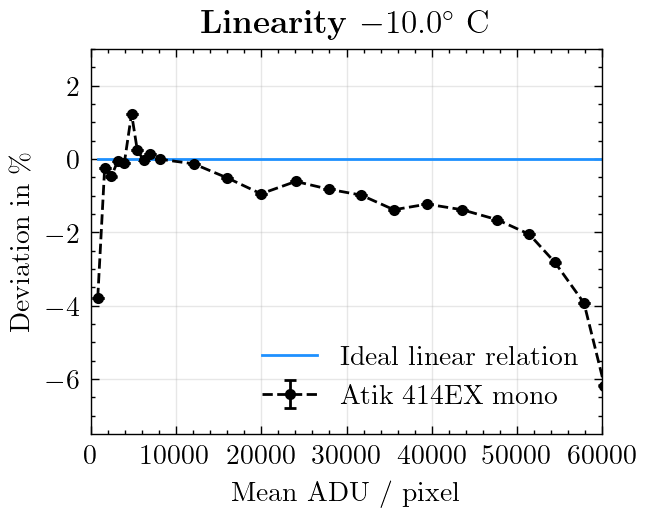
\includegraphics[width=0.65\textwidth]{linearity_zoom.png}
			\caption{A plot of the percentage deviation from ideal linearity, computed from equation \ref{eq:fluxcorrect_timecal}, but zoomed in.}
			\label{fig:linearityzoom}
		\end{figure}
		In general it is recommended that the entire linearity curve is acquired at a dimmer light setting, such that the low-ADU regime does not correspond to short exposure times, and the time calibration is of lesser importance. Turning off 'half' of the flourescent light bulbs in the room, resulting in roughly half the intensity of light, cf. figure \ref{fig:linearitydim} and \ref{fig:linearitydimzoom}, confirms the suspection that fluctuations in the low ADU regime are due to the time offset. Now low ADUs correspond to longer exposure times, and the time offset is of lesser importance, since it corresponds to a much smaller fraction of the total exposure time. Our error is hence reduced significantly by choosing a dimmer light source. Qualitatively the non-linearity curve looks very similar, as it should, since in the ADU space we are independent of exposure times. For this data set the exposure times in exposure times
		$[10, 20, \dots 230, 240]$, all in units of seconds, have been used. There were however faults in the series of $40s, 50s$ and $60s$, that have been omitted in the analysis. This was due to all of the lights having been turned on in the room by accident, during the acquisition of those datapoints.
		\begin{figure}
			\centering			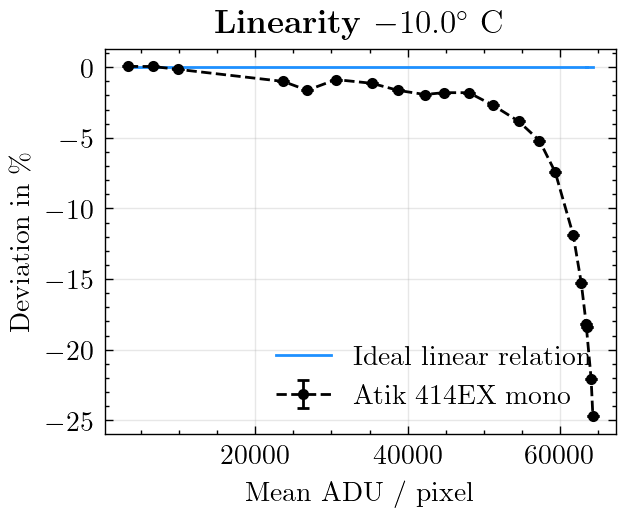
\includegraphics[width=0.65\textwidth]{linearity_dimmed.png}
			\caption{A plot of the percentage deviation from ideal linearity, computed from equation \ref{eq:fluxcorrect_timecal}. Here the data is using a dimmer light source of roughly half the intensity, in order to decouple the low ADU regime from a low exposure time regime, such that the time offset becomes of lesser importance.}
			\label{fig:linearitydim}
		\end{figure}
	\begin{figure}
		\centering			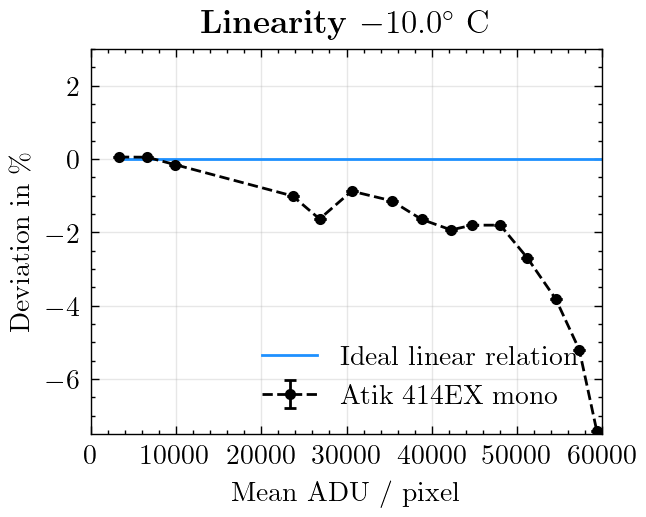
\includegraphics[width=0.65\textwidth]{linearity_zoom_dimmed.png}
		\caption{A plot of the percentage deviation from ideal linearity, computed from equation \ref{eq:fluxcorrect_timecal}, with a dimmed lightsource of roughly half the intensity.}
		\label{fig:linearitydimzoom}
	\end{figure}
		
		\subsection{Shutter test}
		
		\section{Measurement plan}
		This chapter will outline the test procedure measurement plan that results from the conclusions drawn in the preceding chapter. It will be presented as a step by step guide to obtaining the data. 
		
		\subsection{Preparations and corrections}
		\begin{enumerate}
			\item In a dark-room setting, acquire $N=300$ repeats of $0.001s$ exposure images, mean over them to construct the master bias frame
			\item In a lit-room setting acquire $N=300$ $10s$ exposure images of the white screen, mean over them to construct the master flat field frame
			\item In a lit room acquire frames at the exposure times $[0.5s, 1s, 1.5s, \dots, 9s, 9.5s, 10s]$.
			\begin{itemize}
				\item At each exposure time, acquire $N = 10$ repeats that will be meaned over.
				\item For each datapoint acquire a $10s$ reference measurement before and after, to correct for lightsource instability as according to the description outlined above
				\item For each exposure time construct a mean image from repeats
				\item For each of these mean images, one at every exposure time, and the reference measurements respectively before and after:
				\begin{itemize}
					\item Subtract master bias frame from each of the three images.
					\item Set hot pixels equal to mean value of the image, where hot pixels are omitted.
					\item Compute the mean ADU/pixel in each image
					\item Fit a linear relation to the data
					\item Find the roots of the polynomium, which will be interpreted as the temporal offset due to the lack of a shutter
				\end{itemize}
			\end{itemize}
		\end{enumerate}
		
		\subsection{Linearity}
		\begin{enumerate}
			\item Acquire frames at the exposure times
			$[10, 20, \dots 230, 240]$, all in units of seconds.
			\begin{itemize}
				\item At each exposure time, acquire $N = 10$ repeats that will be meaned over.
				\item For each datapoint acquire a $10s$ reference measurement before and after, to correct for lightsource instability as according to the description outlined above
			\end{itemize}
			\item For each exposure time construct a mean image from repeats
			\item For each of these mean images, one at every exposure time, and the reference measurements respectively before and after:
			\begin{itemize}
				\item Subtract master bias frame from each of the three images.
				\item Set hot pixels equal to mean value of the image, where hot pixels are omitted.
				\item Compute the mean ADU/pixel in each image
				\item Compute the non-linearity according to equation \ref{eq:fluxcorrect_timecal}
			\end{itemize}
		\end{enumerate}
		
		This produces a plot like figure \ref{fig:linearity}
		
		\subsection{Temperature dependence of noise}\label{sec:rondc}
		For each temperature in the series $[-10, -8, -6, -4, -2, 0, 2, 4, 6, 8, 10, 12, 14, 16, 18, 20]$:
			\begin{itemize}
				\item $100$ bias frames at $0.001$s used to compute the readout noise as a function of temperature
				\begin{itemize}
					\item At every temperature setpoint consider each repeat image in turn, compute the mean ADU/pixel and subtract it form every pixel in the image
					\item The resultant image is a stochastic gaussian distribution with mean zero
					\item Multiply every pixel with the camera gain, to convert to number of electrons.
					\item Compute the standard deviation from the flattened array of pixels.
					\item This yields $100$ standard deviations, and from this a RMS value can be computed. These values can then be plotted as a function of temperature.
				\end{itemize} 
				\item $100$ dark frames at $10.0s$
				\begin{itemize}
					\item For each temperature sequence, construct a mean image, in order to reduce the readout noise contamination in the image
					\item Subtract the master bias frame.
					\item Set hot pixels equal to mean value of the image, where hot pixels are omitted.
					\item Multiply every pixel with the camera gain, to convert to number of electrons.
					\item Divide every pixel with the exposure time
					\item Compute mean ADU/pixel
				\end{itemize}
			\end{itemize}
		The result of these two analysis may be seen plotted in figure \ref{fig:noise}	
		
\end{document}